\section*{Notas Históricas}

\begin{frame}[plain]
    \fullimg{./imgs/fig1-what-is-ml.png}
\end{frame}

\begin{frame}[plain]
    \fullimg{./imgs/fig2-traj-historica.png}
\end{frame}

\begin{frame}
    \frametitle{O que é aprendizado de máquina?}
    \begin{center}
        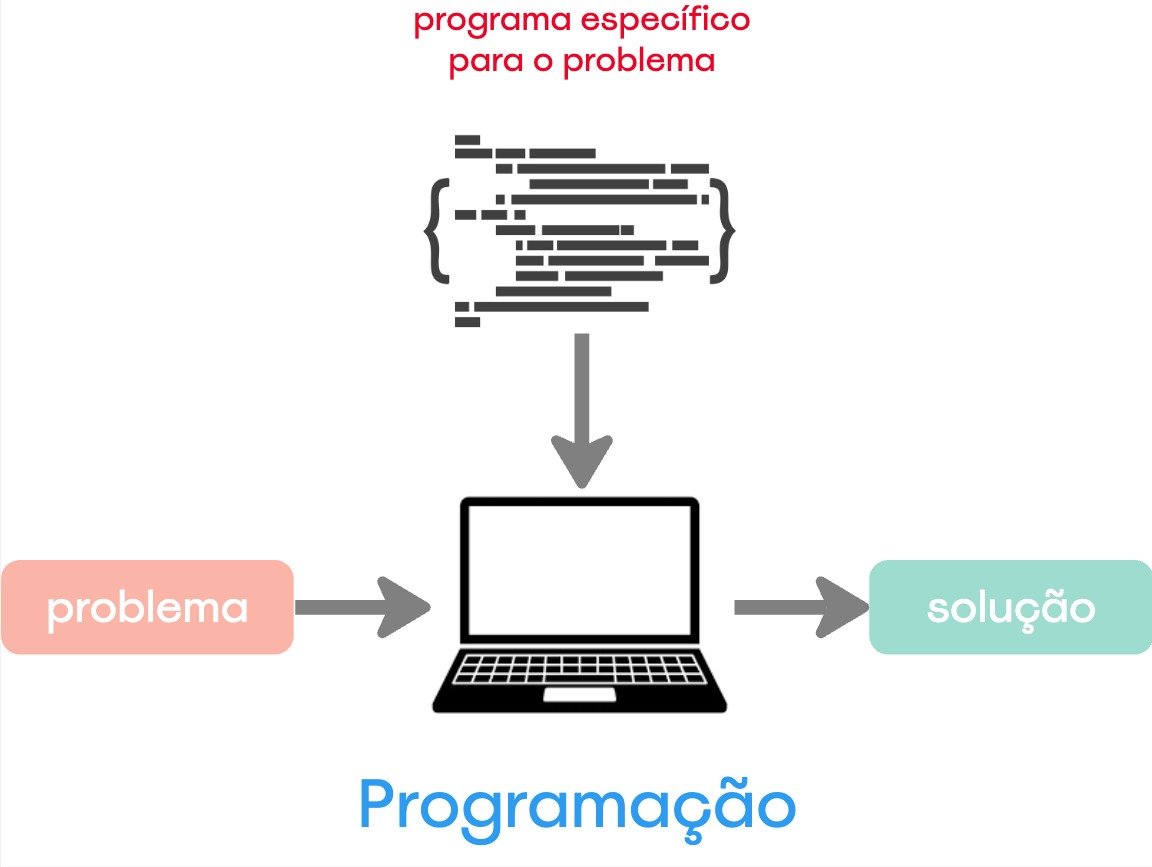
\includegraphics[height=0.4\paperheight]{./imgs/fig3-programacao.jpg}
    \end{center}
    \begin{block}{Programação}
        Cria um programa com uma série de instruções específicamente criadas para para resolver um problema.
    \end{block}
\end{frame}


\subsection{O que é aprendizado de máquina?}
\subsubsection{Programação}

\begin{frame}
    \frametitle{O que é aprendizado de máquina?}
    \begin{center}
        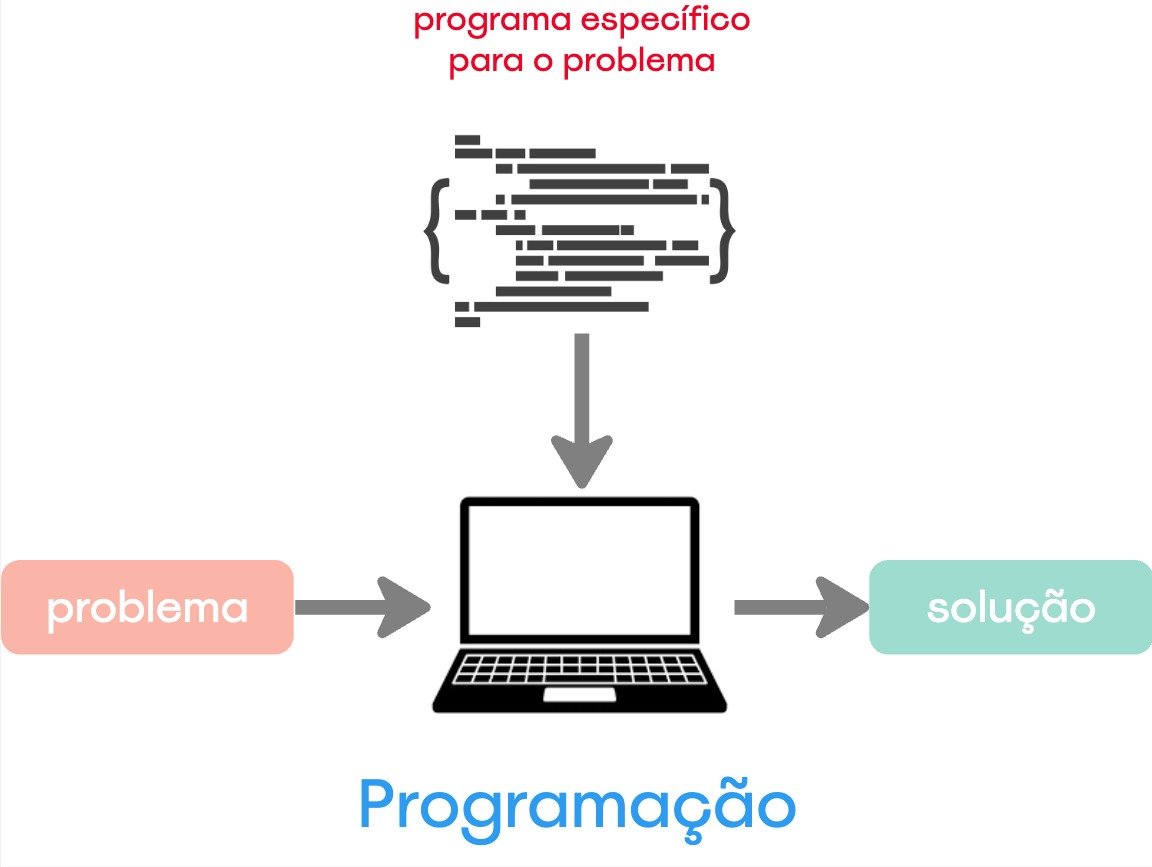
\includegraphics[height=0.4\paperheight]{./imgs/fig3-programacao.jpg}
    \end{center}
    \begin{block}{Programação}
        \begin{itemize}
            \item Problema: prever a posição de um planeta daqui a 150 anos.
            \item Solução: implementa um programa para executar o método numérico para resolver a segunda lei de Newton com as forças envolvidas e as condições iniciais adequadas.
        \end{itemize}            
    \end{block}
\end{frame}

\begin{frame}
    \frametitle{O que é aprendizado de máquina?}
    \begin{center}
        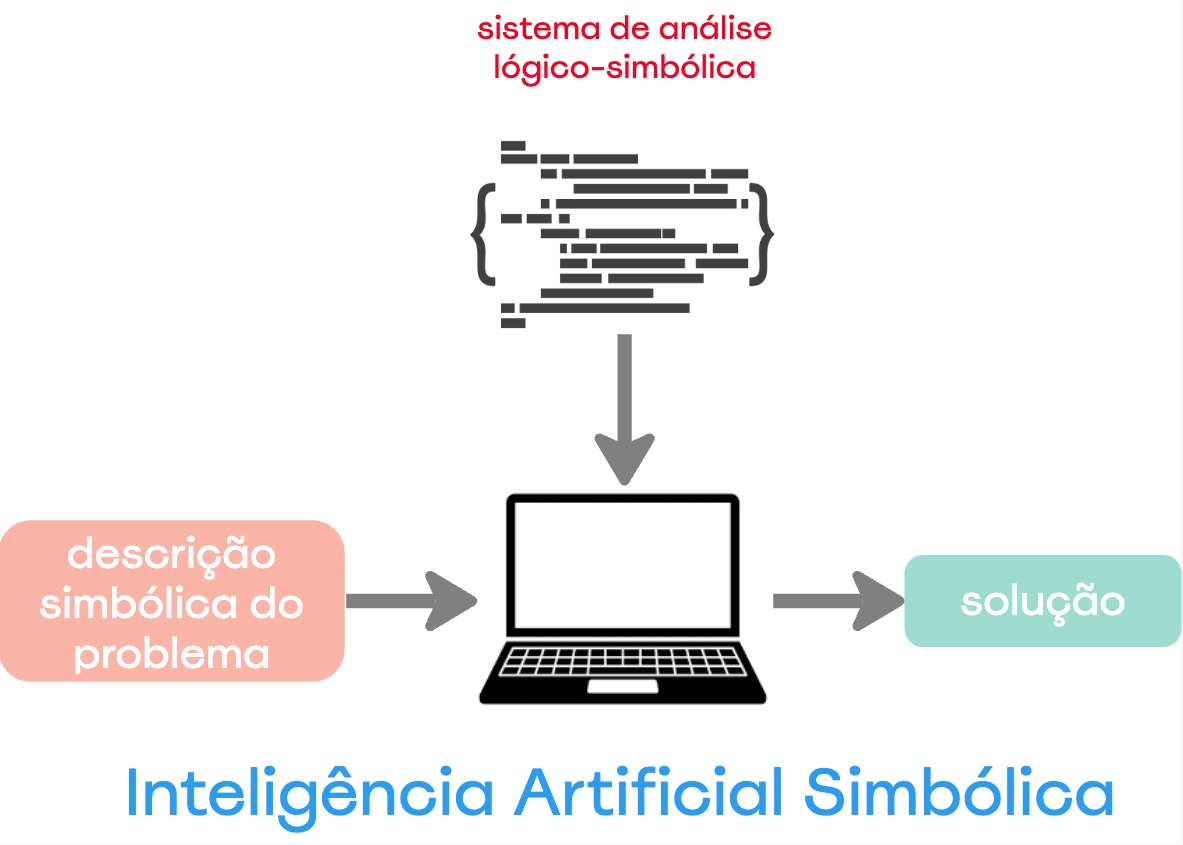
\includegraphics[height=0.4\paperheight]{./imgs/fig4-ai-simbolica.jpg}
    \end{center}
    \begin{block}{IA Simbólica / GOFAI}
        Usa algoritmos de manipulação de expressões lógico-simbólicas para encontrar uma solução dada uma descrição formal do problema.
    \end{block}
\end{frame}

\subsubsection{IA Simbolica}

\begin{frame}
    \frametitle{O que é aprendizado de máquina?}
    \begin{center}
        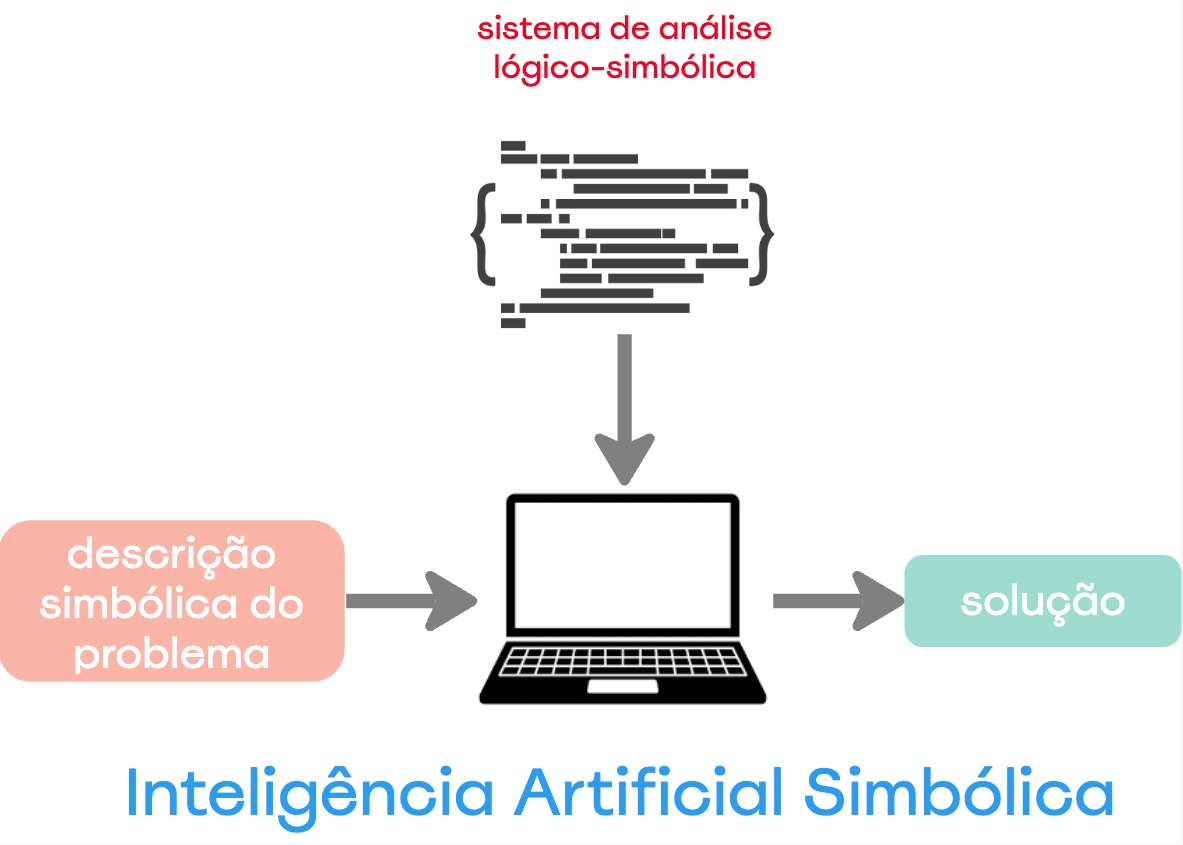
\includegraphics[height=0.4\paperheight]{./imgs/fig4-ai-simbolica.jpg}
    \end{center}
    \begin{block}{IA Simbólica / GOFAI}
        \begin{itemize}
            \item Problema: provar um teorema. 
            \item Solução: um sistema capaz de manipular expressões simbólicas correspondendo a uma série de axiomas 
            e lemas tenta encontrar uma demonstração adequada.
        \end{itemize}            
    \end{block}
\end{frame}


\begin{frame}
    \frametitle{O que é aprendizado de máquina?}
    \begin{center}
        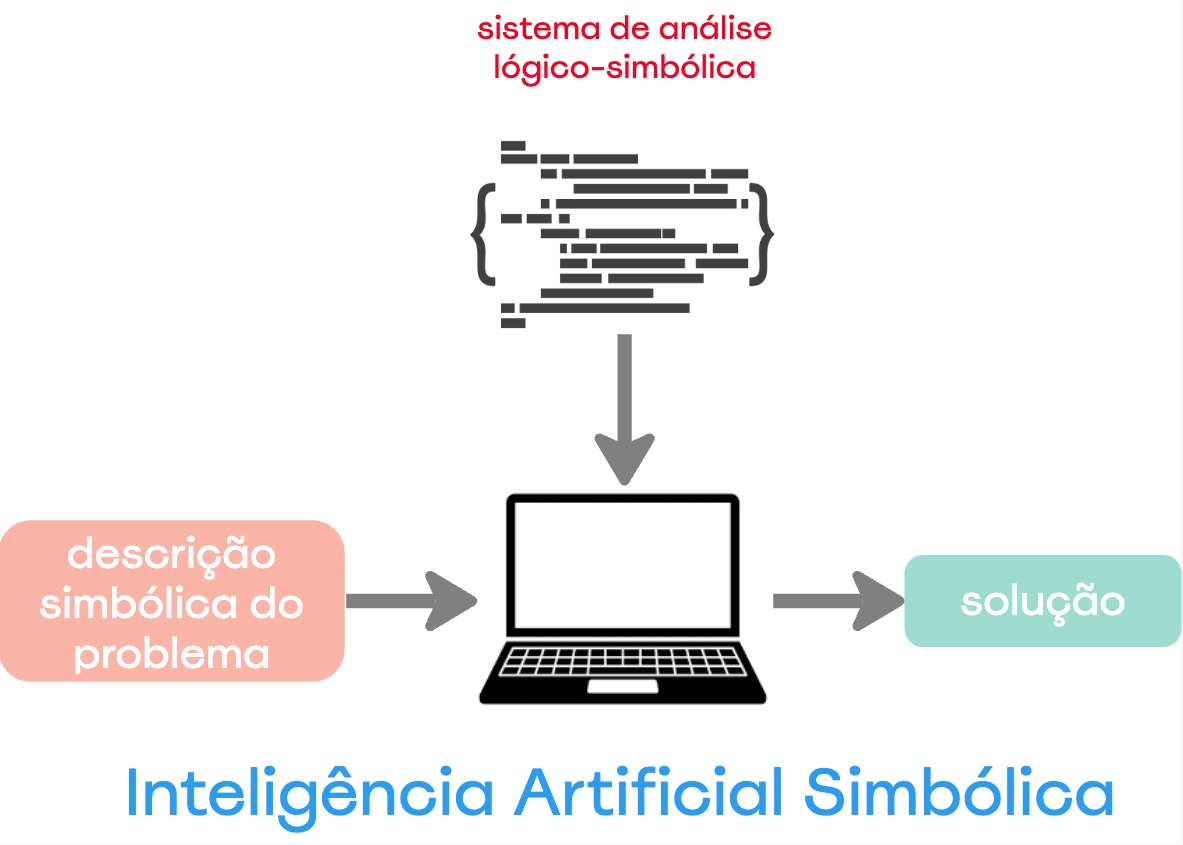
\includegraphics[height=0.4\paperheight]{./imgs/fig4-ai-simbolica.jpg}
    \end{center}
    \begin{block}{IA Simbólica / GOFAI}
        \begin{itemize}
            \item Problema: provar um teorema. 
            \item Solução: um sistema capaz de manipular expressões simbólicas correspondendo a uma série de axiomas 
            e lemas tenta encontrar uma demonstração adequada.
        \end{itemize}            
    \end{block}
\end{frame}

\subsubsection{Aprendizado de Máquina}

\begin{frame}
    \frametitle{O que é aprendizado de máquina?}
    \begin{center}
        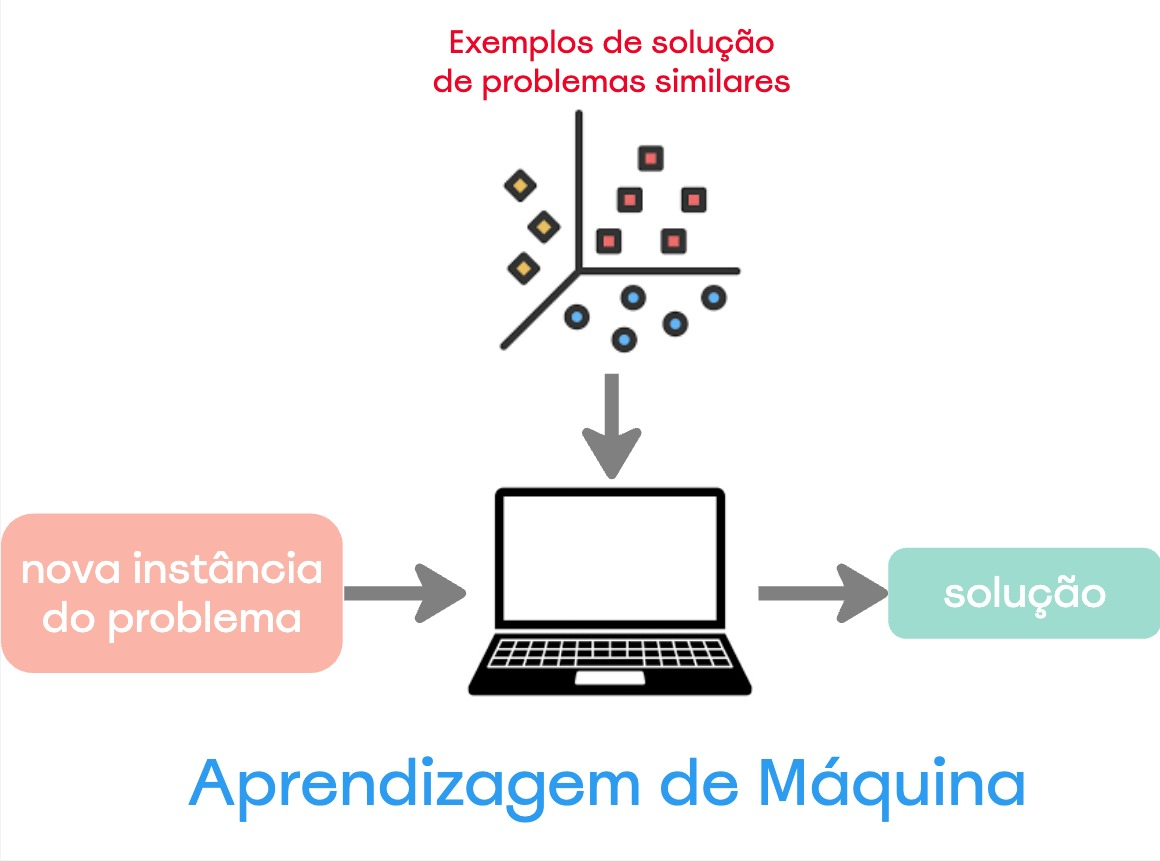
\includegraphics[height=0.4\paperheight]{./imgs/fig5-ml.jpg}
    \end{center}
    \begin{block}{Aprendizado de Máquina}
        dado um conjunto de dados, um algoritmo deriva uma solução que pode ser aplicada para novos dados não vistos. Ex.:
    \end{block}
\end{frame}

\begin{frame}
    \frametitle{O que é aprendizado de máquina?}
    \begin{center}
        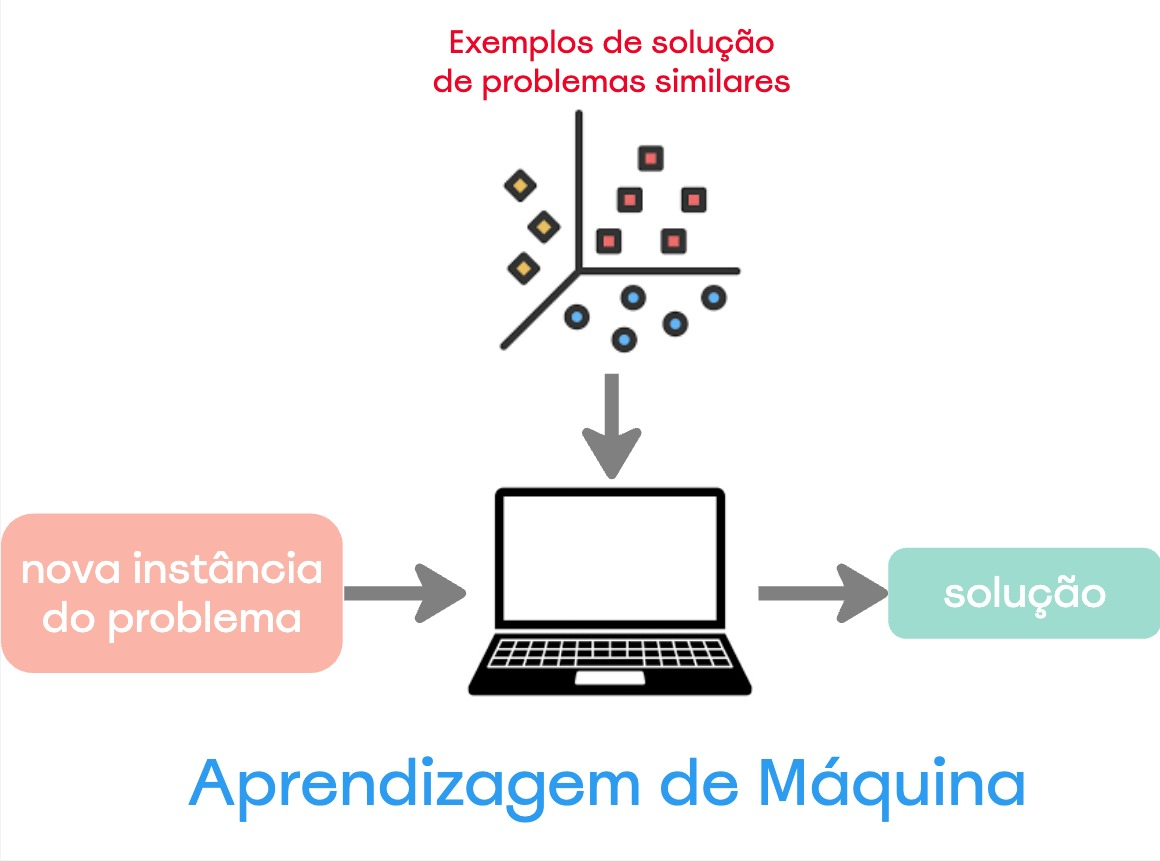
\includegraphics[height=0.4\paperheight]{./imgs/fig5-ml.jpg}
    \end{center}
    \begin{block}{Aprendizado de Máquina}
        \begin{itemize}
            \item Problema: transcrever áudios para texto.
            \item Solução: dado um conjunto de áudios com transcrições conhecidas treinar um algoritmo que é capaz de aprender a fazer a transcrição, e aplicá-lo em novos áudios com transcrição desconhecida.
        \end{itemize}
    \end{block}
\end{frame}

\subsection{Tipos de Aprendizagem de Máquina}

\begin{frame}
    \frametitle{Tipos de Aprendizado – Aprendizado Supervisionado}
    \begin{columns} 
        \column{0.5\textwidth}
        \begin{flushleft}
            Dada uma série de tarefas passadas e suas soluções corretas, o algoritmo deve aprender a resolver a tarefa corretamente em uma situação futura.

            Ex.: classificação, regressão, learn-to-rank, etc. 
                   
        \end{flushleft}
        \column{0.5\textwidth}
        \begin{center}
        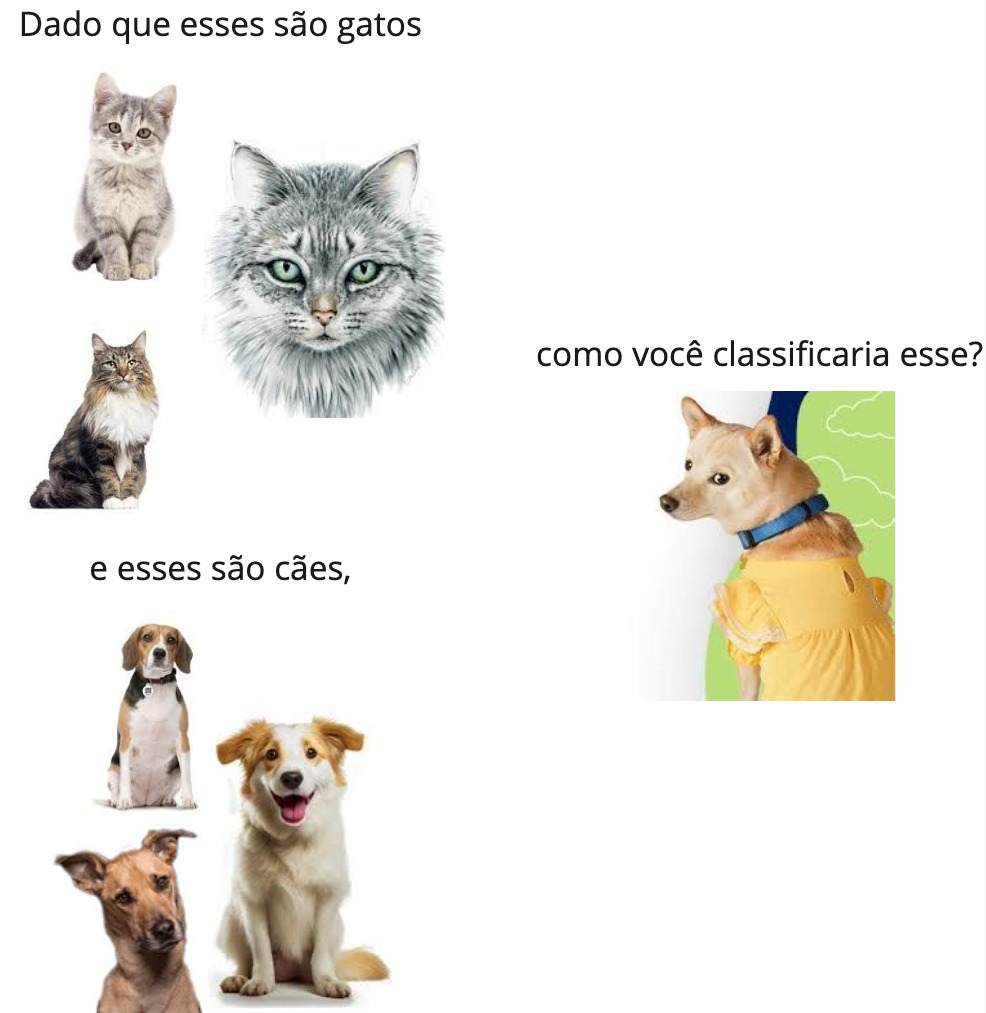
\includegraphics[height=0.6\paperheight]{./imgs/fig6-supervised.jpg}
        \end{center}
    \end{columns}
\end{frame}


\begin{frame}
    \frametitle{Tipos de Aprendizado – Aprendizado Supervisionado}
    \begin{columns} 
        \column{0.5\textwidth}
        \begin{flushleft}
            Dada uma série de tarefas passadas e suas soluções corretas, o algoritmo deve aprender a resolver a tarefa corretamente em uma situação futura.

            Ex.: classificação, regressão, learn-to-rank, etc.                    
        \end{flushleft}
        \column{0.5\textwidth}
        \begin{center}
            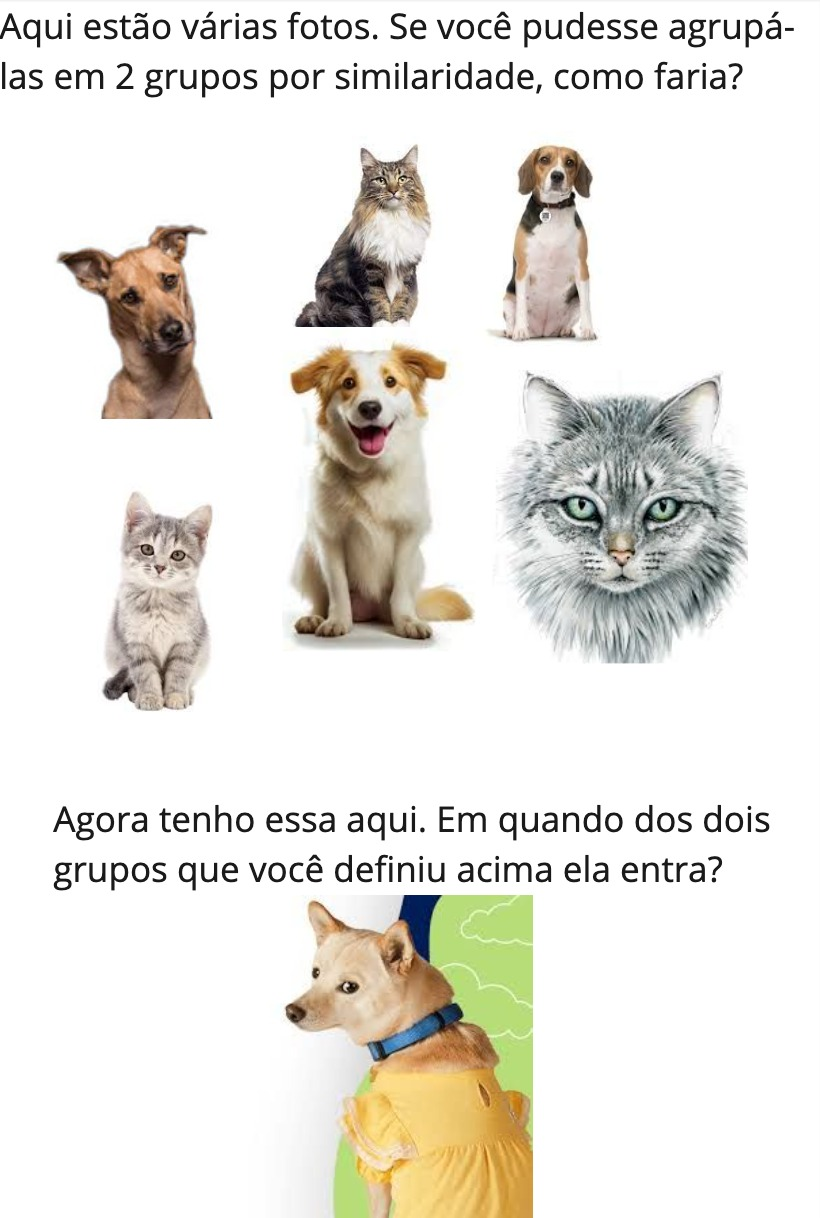
\includegraphics[height=0.6\paperheight]{./imgs/fig7-unsupervised.jpg}
        \end{center}
    \end{columns}
\end{frame}

\begin{frame}
    \frametitle{Tipos de Aprendizado – outros}
    \begin{columns} 
        \column{0.45\textwidth}
        
        \begin{block}{Aprendizado por reforço:}
            \begin{flushleft}
                dado um cenário em que se podem fazer ações e receber recompensas, aprender a fazer as ações que acumulam mais recompensa ao longo das rodadas. Ex.: Alpha Go.    
            \end{flushleft}                    
        \end{block}
        
        \column{0.45\textwidth}
        \begin{block}{Aprendizado Gerativo:}
            \begin{flushleft}
                dado um conjunto de exemplos, aprender a simular a itens da mesma distribuição. Ex.: ChatGPT, Stable Diffusion
            \end{flushleft}
        \end{block}
    \end{columns}
    \vspace{2mm}
    \begin{flushleft}
        \begin{block}{...e muitos outros:}
            aprendizado ativo, aprendizado semi-supervisionado, aprendizado de representações, aprendizado auto-supervisionado, aprendizado estruturado, etc…    
        \end{block}
    \end{flushleft}

\end{frame}